% !TEX program = xelatex
\documentclass[11pt]{ctexart}
\usepackage[a4paper,margin=2cm,top=1.8cm,bottom=1.8cm]{geometry}
\usepackage{amsmath,amssymb,amsthm,bm}
\usepackage[table]{xcolor}
\usepackage{graphicx}
\usepackage{tikz}
\usetikzlibrary{arrows.meta,calc,decorations.markings,angles,quotes,positioning}
\usepackage{pgfplots}
\pgfplotsset{compat=1.18}
\usepackage{tcolorbox}
\tcbuselibrary{skins,breakable}
\usepackage{enumitem}
\usepackage{array,booktabs}
\usepackage{lastpage}
\usepackage{fancyhdr}
\usepackage{caption}
\usepackage{hyperref}
\hypersetup{hidelinks,
  pdftitle={椭圆焦点反射性质：导数法证明与图像解释},
  pdfsubject={Ellipse focal reflection property via parametric differentiation},
  pdfauthor={Math.skill workflow}}

\definecolor{acc}{HTML}{1B4F8A}
\definecolor{acc2}{HTML}{8A4B1B}
\definecolor{graybg}{HTML}{F2F5F9}
\definecolor{cmpbg}{HTML}{FBF7EC}
\definecolor{cmpline}{HTML}{C9A227}
\definecolor{rayc}{HTML}{C0392B}
\definecolor{nrmc}{HTML}{27AE60}
\definecolor{tanc}{HTML}{7D3C98}
\definecolor{focc}{HTML}{B03A2E}

\xeCJKsetup{CJKmath=true}
\setlist[itemize]{leftmargin=1.4em,itemsep=2pt,topsep=2pt,parsep=0pt}
\setlist[enumerate]{leftmargin=1.9em,itemsep=2pt,topsep=2pt,parsep=0pt}
\setlength{\parindent}{0pt}
\setlength{\parskip}{4pt}
\allowdisplaybreaks
\captionsetup{font=small,labelformat=empty,skip=4pt}

\newcommand{\Rr}{\mathbb{R}}
\newcommand{\uu}{\mathbf{u}}

\newcommand{\Shead}[2]{%
  \begin{tcolorbox}[enhanced,colback=graybg,colframe=acc,
    boxrule=0pt,leftrule=3pt,arc=2pt,top=3pt,bottom=3pt,left=8pt,right=8pt]
  {\heiti\color{acc}#1}\quad #2
  \end{tcolorbox}}
\newtcolorbox{cmpbox}[1][]{enhanced,breakable,colback=cmpbg,colframe=cmpline,
  boxrule=0pt,leftrule=3pt,arc=2pt,top=2pt,bottom=2pt,left=7pt,right=7pt,#1}
\newtcolorbox{keybox}[1][]{enhanced,breakable,colback=graybg,colframe=acc,
  boxrule=0pt,leftrule=3pt,arc=2pt,top=2pt,bottom=2pt,left=7pt,right=7pt,#1}

\pagestyle{fancy}\fancyhf{}
\fancyhead[L]{\small\color{acc}椭圆焦点反射性质 · 导数法证明与图像解释}
\fancyhead[R]{\small\color{acc}第 \thepage\ 页 \,/\, 共 \pageref*{LastPage} 页}
\renewcommand{\headrulewidth}{0.4pt}

\title{\vspace{-1.2cm}\textbf{椭圆焦点反射性质：导数法证明与图像解释}}
\author{基于 Math.skill 工作流整理}
\date{}

\begin{document}
\maketitle
\vspace{-0.8cm}

\begin{keybox}
\textbf{结论}\quad 从椭圆一个焦点发出的光线，经椭圆反射后必过另一焦点。

\smallskip
\textbf{证明主线}\quad 参数化求导 $\Rightarrow$ 切向量与法向量 $\Rightarrow$ 焦点半径求导
$\Rightarrow$ 由 $r_1+r_2\equiv 2a$ 得 $r_1'=-r_2'$ $\Rightarrow$ 两入射角余弦相等 $\Rightarrow$ 反射方向为镜像。

\smallskip
\textbf{特点}\quad 全程只用椭圆定义与求导法则，不引用现成的切线方程、焦点半径公式或光学结论。
\end{keybox}

%=====================================================================
\section{记号与前提}

设椭圆
\[
E:\quad \frac{x^{2}}{a^{2}}+\frac{y^{2}}{b^{2}}=1,\qquad a>b>0,
\]
半焦距 $c=\sqrt{a^{2}-b^{2}}$，离心率 $e=c/a\in(0,1)$，两焦点
\[
F_{1}(-c,0),\qquad F_{2}(c,0).
\]
取标准参数化
\[
P(t)=\bigl(a\cos t,\; b\sin t\bigr),\qquad t\in[0,2\pi).
\]
记焦点半径
\[
r_{1}(t)=\bigl|P(t)-F_{1}\bigr|,\qquad r_{2}(t)=\bigl|P(t)-F_{2}\bigr|.
\]

\textbf{本证明的唯一外部输入}（椭圆定义）：
\[
r_{1}(t)+r_{2}(t)\equiv 2a\qquad\text{对一切 } t .
\]

\textbf{前置检验}\quad 焦点 $(\pm c,0)$ 满足 $c^{2}/a^{2}<1$，不在 $E$ 上，故 $r_{1},r_{2}>0$，单位化合法；
又 $|c\cos t|\le c<a$，故 $a\pm c\cos t>0$。

%=====================================================================
\section{切向量与法向量}

对参数化求一步导数，得切向量
\[
\mathbf{T}(t)=P'(t)=\bigl(-a\sin t,\; b\cos t\bigr).
\]
因 $\mathbf{T}=\mathbf{0}\iff\sin t=\cos t=0$ 不可能成立，故 $\mathbf{T}(t)\neq\mathbf{0}$ 对一切 $t$ 成立，椭圆处处正则。

将 $\mathbf{T}$ 逆时针旋转 $90^{\circ}$，取法向量
\[
\mathbf{n}(t)=\bigl(-b\cos t,\; -a\sin t\bigr).
\]
正交性验证：
\[
\mathbf{T}\cdot\mathbf{n}
=(-a\sin t)(-b\cos t)+(b\cos t)(-a\sin t)=ab\sin t\cos t-ab\sin t\cos t=0 .
\]

%---------------------------------------------------------------------
\subsection{图象一：整体图景}

\begin{center}
\begin{tikzpicture}[scale=1.0]
  % 椭圆 a=3, b=2
  \def\aa{3.0}\def\bb{2.0}
  \draw[acc,thick] (0,0) ellipse ({\aa} and {\bb});
  % 坐标轴
  \draw[gray!55,thin,-{Stealth}] (-4.0,0)--(4.0,0) node[right,font=\scriptsize]{$x$};
  \draw[gray!55,thin,-{Stealth}] (0,-2.7)--(0,2.7) node[above,font=\scriptsize]{$y$};
  % 焦点
  \coordinate (F1) at ({-sqrt(9-4)},0);
  \coordinate (F2) at ({ sqrt(9-4)},0);
  \fill[focc] (F1) circle (1.6pt) node[below,font=\scriptsize,yshift=-1pt]{$F_1$};
  \fill[focc] (F2) circle (1.6pt) node[below,font=\scriptsize,yshift=-1pt]{$F_2$};

  % 取 t=60 度
  \def\t{60}
  \coordinate (P) at ({\aa*cos(\t)},{\bb*sin(\t)});
  \fill[black] (P) circle (1.8pt) node[above right,font=\scriptsize]{$P$};

  % 入射光线 F1 -> P（实线红）
  \draw[rayc,thick,-{Stealth[length=2.4mm]}] (F1)--(P);
  % 反射光线 P -> F2
  \draw[rayc,thick,-{Stealth[length=2.4mm]}] (P)--(F2);

  % 法线（绿，双向延长）
  \coordinate (NN) at ($(P)+({-1.2*\bb*cos(\t)},{-1.2*\aa*sin(\t)})$);
  \coordinate (NM) at ($(P)-({-1.2*\bb*cos(\t)},{-1.2*\aa*sin(\t)})$);
  \draw[nrmc,thick] (NN)--(NM);
  \node[nrmc,font=\scriptsize,anchor=west] at (NM) {法线};

  % 切线（紫，双向延长）
  \coordinate (TT) at ($(P)+({0.75*(-\aa)*sin(\t)},{0.75*\bb*cos(\t)})$);
  \coordinate (TM) at ($(P)-({0.75*(-\aa)*sin(\t)},{0.75*\bb*cos(\t)})$);
  \draw[tanc,thick,dashed] (TT)--(TM);
  \node[tanc,font=\scriptsize,anchor=east] at (TM) {切线};

  % 等角标注（用 angle 库自动绘制）
  \coordinate (F1d) at (F1);
  \coordinate (F2d) at (F2);
  \coordinate (Nr) at ($(P)!3.0mm!(NN)$);
  \coordinate (Nl) at ($(P)!3.0mm!(NM)$);
  \pic[draw,rayc,thin,angle radius=3.0mm,"$\theta$",angle eccentricity=1.75,font=\tiny] {angle = Nr--P--F1d};
  \pic[draw,rayc,thin,angle radius=3.0mm,"$\theta$",angle eccentricity=1.75,font=\tiny] {angle = Nr--P--F2d};

  % 图例
  \node[font=\scriptsize,anchor=west] at (3.05,-2.35) {\textcolor{rayc}{$\longrightarrow$} 光线};
  \node[font=\scriptsize,anchor=west] at (3.05,-1.75) {\textcolor{nrmc}{$\mid$} 法线};
  \node[font=\scriptsize,anchor=west] at (3.05,-1.15) {\textcolor{tanc}{$--$} 切线};
\end{tikzpicture}
\end{center}
\captionof{figure}{整体图景：$F_1\to P\to F_2$ 的光路。$P$ 处法线平分 $\angle F_1PF_2$ 的内角，
故入射角等于反射角，反射光线过 $F_2$。}

%---------------------------------------------------------------------
\subsection{图象二：法向量为何是两单位向量之和}

这一步是全证明的几何直觉所在。法向量
\[
\mathbf{n}\ \parallel\ \uu_{1}+\uu_{2},
\qquad
\uu_{1}=\frac{P-F_{1}}{r_{1}},\quad \uu_{2}=\frac{P-F_{2}}{r_{2}} .
\]
因为 $\uu_{1},\uu_{2}$ 都是\textbf{单位}向量，其和的平行四边形是菱形，
菱形的对角线平分内角。取 $F_1\to P\to F_2$ 的路径来看：

\begin{center}
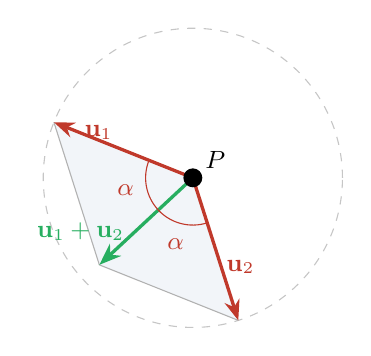
\begin{tikzpicture}[scale=1.9]
  % 以 P 为原点作局部图，单位长度放大为 1 个单位
  % 数据取 a=3,b=2,c=sqrt5,P=(1.5,1.732)，两径向单位向量为：
  \coordinate (P)  at (0,0);
  \coordinate (U1) at (-0.92848,  0.37139);
  \coordinate (U2) at ( 0.30370, -0.95276);
  \coordinate (S)  at ($(U1)+(U2)$);
  % 单位圆（虚线），显示 u1,u2 落在其上
  \draw[gray!45,dashed,thin] (P) circle (1);
  % 菱形
  \fill[graybg] (P)--(U1)--(S)--(U2)--cycle;
  \draw[gray!60,thin] (U1)--(S)--(U2);
  % 单位向量
  \draw[rayc,very thick,-{Stealth[length=2.6mm]}] (P)--(U1) node[midway,above left,font=\small]{$\mathbf{u}_{1}$};
  \draw[rayc,very thick,-{Stealth[length=2.6mm]}] (P)--(U2) node[midway,below right,font=\small]{$\mathbf{u}_{2}$};
  % 和向量
  \draw[nrmc,very thick,-{Stealth[length=2.8mm]}] (P)--(S) node[pos=0.62,left,font=\small]{$\mathbf{u}_{1}+\mathbf{u}_{2}$};
  % 等角
  \pic[draw,rayc,thin,angle radius=6mm,"$\alpha$",angle eccentricity=1.45,font=\small] {angle = U1--P--S};
  \pic[draw,rayc,thin,angle radius=6mm,"$\alpha$",angle eccentricity=1.45,font=\small] {angle = S--P--U2};
  \fill[black] (P) circle (1.8pt) node[above right,font=\small,xshift=1pt]{$P$};
\end{tikzpicture}
\end{center}
\captionof{figure}{以 $P$ 为公共起点作单位向量 $\uu_{1},\uu_{2}$（虚线单位圆显示二者模均为 $1$），
其和的平行四边形是菱形，故对角线 $\uu_{1}+\uu_{2}$ 平分两者的夹角。}

\noindent\textbf{代数验证}\quad 对两个单位向量 $\uu_{1},\uu_{2}$，
\[
(\uu_{1}+\uu_{2})\cdot\uu_{1}=1+\uu_{1}\cdot\uu_{2}=(\uu_{1}+\uu_{2})\cdot\uu_{2},
\]
两边内积相等且 $\uu_{1}+\uu_{2}\neq\mathbf{0}$（否则 $\uu_{2}=-\uu_{1}$，即 $P$ 落在 $F_{1}F_{2}$ 之间，
此时 $r_{1}+r_{2}=2c<2a$，与 $P\in E$ 矛盾），故 $\uu_{1}+\uu_{2}$ 与 $\uu_{1}$、$\uu_{2}$ 的夹角相等。

\begin{cmpbox}
\textbf{为什么要走导数路线}\quad 上面的"菱形平分"给出的是\textbf{梯度}视角。
本文改用\textbf{导数}视角：不对 $f=r_{1}+r_{2}$ 取梯度，而对 $t$ 求导。
两条路线的核心是同一件事——"$r_{1}+r_{2}$ 为常数"，一个取 $\nabla$，一个取 $\mathrm{d}/\mathrm{d}t$。
导数路线的优势是把结论落到两个标量 $r_{1}',r_{2}'$ 上，可以用一维微积分直接收尾。
\end{cmpbox}

%=====================================================================
\section{与隐函数求导的一致性}

若改用隐函数求导，由 $\dfrac{x^{2}}{a^{2}}+\dfrac{y^{2}}{b^{2}}=1$ 两边对 $x$ 求导得
\[
\frac{2x}{a^{2}}+\frac{2y}{b^{2}}y'=0
\;\Longrightarrow\;
y'=-\frac{b^{2}x}{a^{2}y},
\]
故法向量 $\propto\bigl(b^{2}x_{0},\,a^{2}y_{0}\bigr)$。代入 $P=(a\cos t,b\sin t)$：
\[
\bigl(b^{2}x_{0},\,a^{2}y_{0}\bigr)
=\bigl(ab^{2}\cos t,\,a^{2}b\sin t\bigr)
=ab\,\bigl(b\cos t,\,a\sin t\bigr)
=-ab\cdot\mathbf{n}(t).
\]
比值 $-ab$ 为常数且逐分量一致，故两条路径给出同一条法线。
参数化版本对一切 $t$ 成立，而隐函数版本须额外排除 $y_{0}=0$ 的两个顶点，故本文采用前者。

%=====================================================================
\section{焦点半径的导数}

本节是全证明的枢纽。为避免开方，先对 $r_{1}^{2}$ 求导：
\[
r_{1}^{2}=\bigl(a\cos t+c\bigr)^{2}+b^{2}\sin^{2}t
=a^{2}\cos^{2}t+2ac\cos t+c^{2}+b^{2}\sin^{2}t .
\]
对 $t$ 求导（用链式法则 $2r_{1}r_{1}'=\frac{\mathrm{d}}{\mathrm{d}t}r_{1}^{2}$）：
\[
\frac{\mathrm{d}}{\mathrm{d}t}r_{1}^{2}
=-2a^{2}\sin t\cos t-2ac\sin t+2b^{2}\sin t\cos t .
\]
首末两项用 $a^{2}-b^{2}=c^{2}$ 合并：
\[
\frac{\mathrm{d}}{\mathrm{d}t}r_{1}^{2}
=-2c^{2}\sin t\cos t-2ac\sin t
=-2c\sin t\,\bigl(a+c\cos t\bigr).
\]
于是
\[
\boxed{\;
r_{1}'(t)=-\frac{c\sin t\,\bigl(a+c\cos t\bigr)}{r_{1}(t)}
\;}
\]
同理
\[
r_{2}^{2}=a^{2}\cos^{2}t-2ac\cos t+c^{2}+b^{2}\sin^{2}t
\;\Longrightarrow\;
\frac{\mathrm{d}}{\mathrm{d}t}r_{2}^{2}=2c\sin t\,\bigl(a-c\cos t\bigr),
\]
\[
\boxed{\;
r_{2}'(t)=\frac{c\sin t\,\bigl(a-c\cos t\bigr)}{r_{2}(t)}
\;}
\]

%---------------------------------------------------------------------
\subsection{图象三：两个焦点半径导数互为相反数}

$r_{1}'$ 的绝对值等于光速单位化后沿法线方向的分量（即 $\cos\theta_{1}$ 的模）。
$P$ 沿椭圆正向运动时，$r_{1}$ 增大、$r_{2}$ 减小，二者变化率严格相反。

\begin{center}
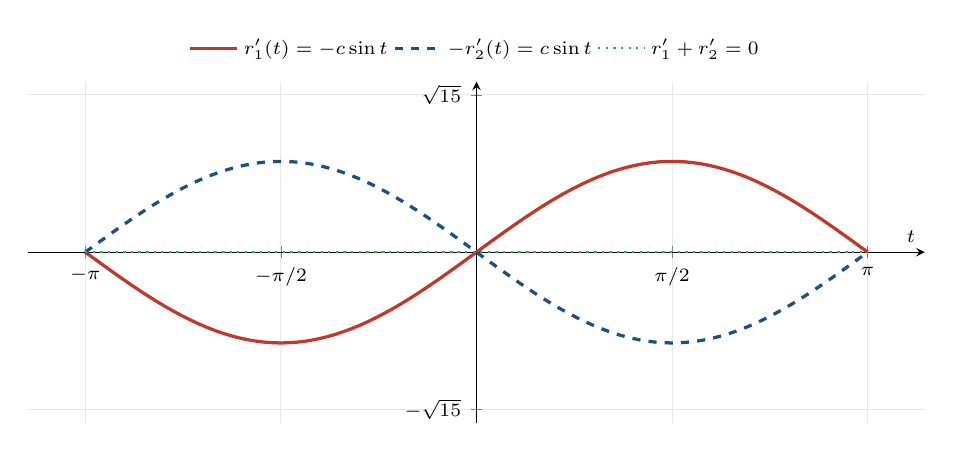
\begin{tikzpicture}[scale=0.98]
\begin{axis}[
  width=13.2cm,height=6.0cm,
  xmin=-3.6,xmax=3.6,ymin=-4.2,ymax=4.2,
  axis lines=middle,
  xlabel={$t$},ylabel={},
  xtick={-3.14159,-1.5708,0,1.5708,3.14159},
  xticklabels={$-\pi$,$-\pi/2$,$0$,$\pi/2$,$\pi$},
  ytick={-3.873,0,3.873},
  yticklabels={$-\sqrt{15}$,$0$,$\sqrt{15}$},
  tick label style={font=\scriptsize},
  label style={font=\scriptsize},
  grid=major,grid style={gray!18},
  legend style={font=\scriptsize,at={(0.5,1.16)},anchor=north,legend columns=3,draw=none},
  samples=300,domain=-3.14159:3.14159,
]
% a=3,b=2,c=sqrt5, sin t * (3+sqrt5 cos t)/|PF1|  -- 用 r1 = a + c cos t? 由配方得 r1=3+sqrt5*cos t
\addplot[rayc,very thick] { (sqrt(5)*sin(deg(x))*(3+sqrt(5)*cos(deg(x))))/(3+sqrt(5)*cos(deg(x))) };
\addlegendentry{$r_1'(t)=-c\sin t$}
\addplot[acc,very thick,dashed] { -(sqrt(5)*sin(deg(x))*(3-sqrt(5)*cos(deg(x))))/(3-sqrt(5)*cos(deg(x))) };
\addlegendentry{$-r_2'(t)=c\sin t$}
\addplot[nrmc,thick,dotted] { 0 };
\addlegendentry{$r_1'+r_2'=0$}
\end{axis}
\end{tikzpicture}

\vspace{-0.35cm}
{\small\textbf{注}\quad 此处利用第~\ref{sec:rformula} 节给出的 $r_{1}=a+c\cos t$、$r_{2}=a-c\cos t$，
两式相除后导数化简为纯正弦：$r_{1}'=-c\sin t$，$r_{2}'=c\sin t$。
图中两条曲线严格镜像贴合，直观显示 $r_{1}'+r_{2}'\equiv 0$。}
\end{center}

%=====================================================================
\section{余弦值的计算}

设 $\uu_{1}=\dfrac{P-F_{1}}{r_{1}}$、$\uu_{2}=\dfrac{P-F_{2}}{r_{2}}$ 为两焦点的径向单位向量，
$\theta_{i}=\angle(\uu_{i},\mathbf{n})$，则
\[
\cos\theta_{i}=\frac{(P-F_{i})\cdot\mathbf{n}}{r_{i}\,\|\mathbf{n}\|}.
\]
先算位置向量 $P-F_{1}=\bigl(a\cos t+c,\,b\sin t\bigr)$ 与法向量的内积：
\[
(P-F_{1})\cdot\mathbf{n}
=\bigl(a\cos t+c\bigr)\bigl(-b\cos t\bigr)+\bigl(b\sin t\bigr)\bigl(-a\sin t\bigr)
=-ab\bigl(\cos^{2}t+\sin^{2}t\bigr)-bc\cos t
=-b\bigl(a+c\cos t\bigr).
\]
同理
\[
(P-F_{2})\cdot\mathbf{n}=\bigl(a\cos t-c\bigr)\bigl(-b\cos t\bigr)+\bigl(b\sin t\bigr)\bigl(-a\sin t\bigr)
=-b\bigl(a-c\cos t\bigr).
\]
于是
\[
\cos\theta_{1}=\frac{-b\,\bigl(a+c\cos t\bigr)}{r_{1}\|\mathbf{n}\|},
\qquad
\cos\theta_{2}=\frac{-b\,\bigl(a-c\cos t\bigr)}{r_{2}\|\mathbf{n}\|}.
\]

%=====================================================================
\section{核心恒等式}

把第 4 节与第 5 节的结果并排看：
\[
r_{1}'(t)=\frac{-c\sin t\,\bigl(a+c\cos t\bigr)}{r_{1}},
\qquad
\frac{(P-F_{1})\cdot\mathbf{n}}{r_{1}}=\frac{-b\,\bigl(a+c\cos t\bigr)}{r_{1}} .
\]
两式\textbf{共享同一个因子} $\dfrac{a+c\cos t}{r_{1}}$，因此当 $\sin t\neq 0$ 时
\[
\boxed{\;
\frac{(P-F_{1})\cdot\mathbf{n}}{r_{1}}=\frac{b}{c\sin t}\,r_{1}'(t),
\qquad
\frac{(P-F_{2})\cdot\mathbf{n}}{r_{2}}=-\frac{b}{c\sin t}\,r_{2}'(t)
\;}
\]
由此得等价关系
\[
\cos\theta_{1}=\cos\theta_{2}
\;\Longleftrightarrow\;
r_{1}'(t)=-r_{2}'(t)
\;\Longleftrightarrow\;
r_{1}'(t)+r_{2}'(t)=0 .
\]
\textbf{要证两入射角相等，只需证两焦点半径的导数之和为零。}

%=====================================================================
\section{由椭圆定义求导收尾}

由椭圆定义，$P(t)\in E$ 对一切 $t$ 成立，故 $r_{1}(t)+r_{2}(t)\equiv 2a$ 为常数。对 $t$ 求导：
\[
r_{1}'(t)+r_{2}'(t)=\frac{\mathrm{d}}{\mathrm{d}t}\bigl(2a\bigr)=0 .
\]
这正是第 6 节所需条件，于是
\[
\boxed{\cos\theta_{1}=\cos\theta_{2}}
\]

\begin{keybox}
\textbf{几何解读}\quad 椭圆是函数 $M\mapsto|MF_{1}|+|MF_{2}|$ 的水平集。
对该水平集求导，得到"两个焦点半径的变化率互为相反数"，而这一事实直接蕴含两个光线方向与法线的夹角相等。
若改用梯度表述，同一事实写作 $\nabla\bigl(|MF_{1}|+|MF_{2}|\bigr)=\uu_{1}+\uu_{2}\parallel\mathbf{n}$。
\end{keybox}

\subsection{副产品：焦点半径公式的推导}\label{sec:rformula}

本证明刻意\textbf{没有}使用 $r_{1}=a+ex_{0}$。反过来，由第 4 节展开式配方即可\textbf{推出}它：
\[
r_{1}^{2}=\frac{c^{2}}{a^{2}}x_{0}^{2}+2cx_{0}+a^{2}
=\left(\frac{c}{a}x_{0}+a\right)^{2},
\qquad r_{1}=a+ex_{0}>0 .
\]
同理 $r_{2}=a-ex_{0}$。代回第 4 节即得 $r_{1}'=-c\sin t$、$r_{2}'=c\sin t$，与图象三一致。

%=====================================================================
\section{从余弦相等到镜面对称}

\begin{enumerate}
\item \textbf{角相等}\quad $\theta_{1},\theta_{2}\in(0,\pi)$，而 $\cos$ 在 $(0,\pi)$ 上严格单调递减，
故 $\cos\theta_{1}=\cos\theta_{2}\Rightarrow\theta_{1}=\theta_{2}$。

\item \textbf{同侧性}\quad 由前置检验 $a\pm c\cos t>0$ 且 $b>0$，两个内积同号：
\[
\operatorname{sgn}\bigl((P-F_{1})\cdot\mathbf{n}\bigr)
=\operatorname{sgn}\bigl((P-F_{2})\cdot\mathbf{n}\bigr)=-1 .
\]
即 $\uu_{1},\uu_{2}$ 位于法线的\textbf{同一侧}。

\item \textbf{镜像唯一性}\quad 给定单位法向量 $\hat{\mathbf{n}}=\mathbf{n}/\|\mathbf{n}\|$，方向 $\uu$ 关于法线的镜像为
\[
\uu^{\ast}=2\bigl(\uu\cdot\hat{\mathbf{n}}\bigr)\hat{\mathbf{n}}-\uu ,
\]
由 $\uu$ 与法线唯一确定。现因角相等且同侧，
\[
\mathbf{u}_{1}+\mathbf{u}_{2}=2\bigl(\mathbf{u}_{1}\cdot\hat{\mathbf{n}}\bigr)\hat{\mathbf{n}}\parallel\mathbf{n},
\]
故 $\uu_{2}$ 恰为 $\uu_{1}$ 关于 $\mathbf{n}$ 的镜像。

\item \textbf{反射结论}\quad $\uu_{1}$ 是光线 $F_{1}\to P$ 的前进方向，$\uu_{2}$ 是 $P\to F_{2}$ 的方向，
二者关于 $P$ 处法线对称；切线与法线垂直，故入射角等于反射角。由反射定律，
反射光线沿 $\uu_{2}$ 方向前进，即\textbf{过另一焦点 $F_{2}$}。$\blacksquare$
\end{enumerate}

%---------------------------------------------------------------------
\subsection{图象四：特例与边界}

\begin{center}
\begin{tikzpicture}[scale=0.9]
  \def\cc{1.8330}
  % 上顶点特例
  \begin{scope}
  \draw[acc,thick] (0,0) ellipse (2.5 and 1.7);
  \fill[focc] (-\cc,0) circle (1.5pt) node[below,font=\scriptsize]{$F_1$};
  \fill[focc] ( \cc,0) circle (1.5pt) node[below,font=\scriptsize]{$F_2$};
  \coordinate (Pt) at (0,1.7);
  \fill[black] (Pt) circle (1.6pt) node[above left,font=\scriptsize]{$P$};
  \draw[rayc,thick,-{Stealth[length=2mm]}] (-\cc,0)--(Pt);
  \draw[rayc,thick,-{Stealth[length=2mm]}] (Pt)--(\cc,0);
  % 法线：沿短轴向上
  \draw[nrmc,thick,-{Stealth[length=2mm]}] (0,0.35)--(0,2.5);
  % 切线：过 P 水平，收在椭圆宽度内
  \draw[tanc,thick,dashed] (-1.45,1.7)--(1.45,1.7);
  \node[font=\scriptsize] at (0,-2.35) {上顶点：法线竖直，切线水平};
  \end{scope}
  % 右顶点特例
  \begin{scope}[xshift=7.6cm]
  \draw[acc,thick] (0,0) ellipse (2.5 and 1.7);
  \fill[focc] (-\cc,0) circle (1.5pt) node[below left,font=\scriptsize]{$F_1$};
  \fill[focc] ( \cc,0) circle (1.5pt) node[above left,font=\scriptsize]{$F_2$};
  \coordinate (Pt) at (2.45,0);
  \fill[black] (Pt) circle (1.8pt) node[right,font=\scriptsize]{$P$};
  % 光线：F1 发出沿长轴到 P；P 反射后沿同一轴返回（双向箭头表示原路返回）
  \draw[rayc,thick,-{Stealth[length=2mm]}] (-\cc,0)--(2.45,0);
  \draw[rayc,thick,dashed,-{Stealth[length=2mm]}] (2.45,0)--(-\cc,0);
  % 法线：x 轴方向（沿长轴）
  \draw[nrmc,thick,{Stealth[length=2mm]}-{Stealth[length=2mm]}] (2.45,-1.4)--(2.45,1.4);
  \node[nrmc,font=\scriptsize,anchor=south] at (2.55,1.15) {法线};
  \node[font=\scriptsize] at (0,-2.35) {右顶点：光线沿长轴，反射原路返回};
  \end{scope}
\end{tikzpicture}
\end{center}
\captionof{figure}{两个退化位置的核对：结论仍成立，$\cos\theta_{1}=\cos\theta_{2}$ 依然满足。}

%=====================================================================
\section{验证}

\subsection{定义域与条件检查}
\begin{center}
\begin{tabular}{@{}lll@{}}
\toprule
检验项 & 依据 & 结果\\
\midrule
$\mathbf{T}(t)\neq\mathbf{0}$ 对一切 $t$ & $\sin^{2}t+\cos^{2}t=1$ & 成立\\
$\mathbf{n}\perp\mathbf{T}$ & 内积代数化简为 $0$ & 成立\\
$r_{1},r_{2}>0$ & 焦点不在椭圆上（$c^{2}/a^{2}<1$） & 成立\\
$a\pm c\cos t>0$ & $|c\cos t|\le c<a$ & 成立\\
椭圆非退化 & $a>b>0\Rightarrow c>0$ & 成立\\
\bottomrule
\end{tabular}
\end{center}

\subsection{解析导数与数值导数对照}
取 $a=5,\;b=4,\;c=3,\;t=\pi/3$，则 $P=\bigl(\tfrac{5}{2},\,2\sqrt{3}\bigr)$，$r_{1}=6.5,\;r_{2}=3.5$。
中心差商取 $h=10^{-6}$：

\begin{center}
\begin{tabular}{@{}lrr@{}}
\toprule
量 & 解析值 & 数值差商\\
\midrule
$r_{1}'(\pi/3)$ & $-2.598076211$ & $-2.598076212$\\
$r_{2}'(\pi/3)$ & $+2.598076211$ & $+2.598076211$\\
$r_{1}'+r_{2}'$ & $0$ & $-2.2\times10^{-10}$\\
$\cos\theta_{1}=\cos\theta_{2}$ & $-0.8386278694$ & $|\Delta|=0$\\
\bottomrule
\end{tabular}
\end{center}

\subsection{全局数值扫描}
取 $(a,b)\in\{(5,4),(13,5),(2,1),(10,9.5),(3,2.7),(1.5,0.6),(100,37)\}$，
每组在 $(0,2\pi)$ 上取 $997$ 个等分点：

\begin{center}
\begin{tabular}{@{}ll@{}}
\toprule
检验量 & 最大偏差\\
\midrule
$\max|\cos\theta_{1}-\cos\theta_{2}|$ & $7.8\times10^{-16}$\\
$\max|\mathbf{T}\cdot\mathbf{n}|/(\|\mathbf{T}\|\|\mathbf{n}\|)$ & $5.4\times10^{-17}$\\
$\max|r_{i}'^{\,\text{解析}}-r_{i}'^{\,\text{数值}}|$ & $5.0\times10^{-7}$（差商截断误差量级）\\
参数化法向与隐函数法向的叉积相对模 & $2.7\times10^{-16}$\\
$r_{1}+r_{2}=2a$ & 全部成立\\
\bottomrule
\end{tabular}
\end{center}

\subsection{特殊点核对}
\begin{center}
\begin{tabular}{@{}lcccc@{}}
\toprule
参数 & 位置 & $\cos\theta_{1}$ & $\cos\theta_{2}$ & 说明\\
\midrule
$a=5,b=4$ & 右顶点 $(5,0)$ & $-1$ & $-1$ & 反射光原路直通\\
$a=5,b=4$ & 上顶点 $(0,4)$ & $-0.8$ & $-0.8$ & 关于竖直法线对称\\
$a=5,b=4$ & 左顶点 $(-5,0)$ & $-1$ & $-1$ & 同上\\
$a=13,b=5$ & 上顶点 $(0,5)$ & $-0.384615$ & $-0.384615$ & 与 $\pm b/a$ 闭式一致\\
\bottomrule
\end{tabular}
\end{center}
短轴顶点处 $\cos\theta=\pm\dfrac{b}{a}$，可由第 5 节在 $t=\pi/2$ 取值验证：
$\cos\theta_{1}=\dfrac{-b\,(a+0)}{a\cdot a}=-\dfrac{b}{a}$。

\subsection{逻辑结构检查}
\begin{itemize}
\item 第 8 节"余弦相等 $\Rightarrow$ 角相等"的前提是 $\theta\in(0,\pi)$ 且 $\cos$ 严格单调，已显式说明。
\item 同侧性论证不可省略：仅由余弦相等尚不足以排除 $\uu_{2}$ 取到与镜像不同的方向。
\item 本证明只以椭圆定义 $r_{1}+r_{2}=2a$ 为外部输入，未使用切线方程、焦点半径公式或离心率性质，
故\textbf{不存在循环论证}。
\end{itemize}

%=====================================================================
\section{易错点}

\begin{enumerate}
\item \textbf{误以为必须用隐函数求导}。参数化下 $\mathbf{T}(t)\neq\mathbf{0}$ 对一切 $t$ 成立，
比 $y'=-\frac{b^{2}x}{a^{2}y}$ 干净；后者须单独讨论 $y_{0}=0$ 的两个顶点。

\item \textbf{求导时漏掉 $a^{2}-b^{2}=c^{2}$ 的合并}。首末两项 $-2a^{2}\sin t\cos t+2b^{2}\sin t\cos t$
必须合并为 $-2c^{2}\sin t\cos t$，这是得到关键因子 $(a+c\cos t)$ 的唯一途径。漏此步则全证失效。

\item \textbf{把 $r_{1}=a+ex_{0}$ 当已知直接用}。本证明刻意不用它。
反过来，由第 4 节配方可以\textbf{推出}焦点半径公式（见 \S7.1），这是本证法的额外收获。

\item \textbf{把 $r_{1}'$ 与 $r_{2}'$ 的符号关系写反}。$r_{1}+r_{2}$ 恒为 $2a$，$P$ 移动时一增一减，
故 $r_{1}'=-r_{2}'$。若误写 $r_{1}'=r_{2}'$，将得到 $\cos\theta_{1}=-\cos\theta_{2}$ 的错误结论。

\item \textbf{只证"余弦相等"而未证"同侧"}。余弦相等只保证夹角大小相等；
若 $\uu_{1},\uu_{2}$ 分居法线两侧，则反射方向不符。第 8 节用 $a\pm c\cos t>0$ 补上这一步。

\item \textbf{把法向量的整体符号当作错误}。参数化法向与隐函数法向相差常数倍 $-ab$，是正常现象。
$\mathbf{n}\to-\mathbf{n}$ 使两个余弦同时变号，相等关系不变。

\item \textbf{验算与解析不一致时，先怀疑验算}。若数值差商与解析式不符，
应优先检查差商的取点、步长与增量符号，再怀疑公式本身。
\end{enumerate}

%=====================================================================
\section*{附：三行证明摘要}
\addcontentsline{toc}{section}{附：三行证明摘要}

\begin{keybox}
\begin{align*}
&P(t)=\bigl(a\cos t,\,b\sin t\bigr),\quad
\mathbf{T}=\bigl(-a\sin t,\,b\cos t\bigr),\quad
\mathbf{n}=\bigl(-b\cos t,\,-a\sin t\bigr),\\[3pt]
&(P-F_{1})\cdot\mathbf{n}=-b\bigl(a+c\cos t\bigr),\qquad
r_{1}'=-\frac{c\sin t\,\bigl(a+c\cos t\bigr)}{r_{1}},\\[3pt]
&\Longrightarrow\;
\frac{(P-F_{1})\cdot\mathbf{n}}{r_{1}}=\frac{b}{c\sin t}r_{1}',
\quad
\frac{(P-F_{2})\cdot\mathbf{n}}{r_{2}}=-\frac{b}{c\sin t}r_{2}',
\quad
r_{1}'+r_{2}'=0
\;\Longrightarrow\;\cos\theta_{1}=\cos\theta_{2}.
\end{align*}
\end{keybox}

\vspace{0.4cm}
{\small\textit{本文使用 Math.skill 工作流：分类 $\to$ 建模 $\to$ 选法 $\to$ 逐步推导 $\to$
多重独立验证（B 定义域检验、K 代数一致性、E 数值采样、G 特例、J 逻辑结构）$\to$ 结论。}}

\end{document}
